% Section 7: Results

\section{Results and Analysis}

This section presents results organized to demonstrate: (1) computational scalability enabling real-world deployment, (2) problem feasibility validation, and (3) multi-objective optimization revealing fundamental trade-offs for decision-making.

\subsection{Framework Enables Previously Intractable Scenarios}

Real-world GBSS design requires optimizing networks with 50-100 sensor locations—a scale where exhaustive methods become computationally prohibitive. Table \ref{tab:scalability} quantifies this barrier and demonstrates that our framework's use of meta-heuristic optimization (GA) enables practitioners to solve previously intractable problems.

\begin{table}[h]
\centering
\caption{Computational Tractability: Framework Scalability Demonstration}
\label{tab:scalability}
\begin{tabular}{lcccc}
\toprule
\textbf{Method} & \textbf{Complexity} & \textbf{n=10} & \textbf{n=20} & \textbf{n=88 (Real)} \\
\midrule
\textbf{Exhaustive Search} & $O(2^n)$ & $1,024$ & $1,048,576$ & $3 \times 10^{26}$ \\
 & & Feasible & \textbf{Intractable} & \textbf{Impossible} \\
\midrule
\textbf{MIP/MILP} & NP-hard & Feasible & Challenging & \textbf{Intractable} \\
\midrule
\textbf{Our Framework} & $O(g \times p)$ & 2 min & 2 min & \textbf{2.5 min} \\
 & & \multicolumn{3}{c}{Tractable at all scales} \\
\bottomrule
\end{tabular}
\end{table}

The key insight is not that GA has polynomial complexity (well-established in optimization literature), but rather that combining GA with high-fidelity urban modeling (OSM + ray-tracing) enables city-scale deployment planning for the first time. Prior methods either scale (but lack urban fidelity) or provide fidelity (but don't scale). Our framework achieves both, completing Avenida Paulista optimization (88 locations, 4,921 buildings) in 2.5 minutes—making real-world GBSS planning computationally viable.

\subsection{Problem Feasibility Validation}

Before optimization, we validated that requirements are achievable by activating all available sensors (upper bound analysis). For the synthetic scenario with 10 sensor locations, maximum coverage reached 85.56\% with redundancy of 9.28—exceeding the adjusted requirement of 80\% and confirming the problem is well-posed. This sanity check prevents optimization toward unattainable targets.

\subsection{Multi-Objective Optimization: Pareto Front Analysis}

Rather than evaluating fixed sensor configurations, we employed NSGA-II to discover the Pareto-optimal front representing fundamental trade-offs between coverage, redundancy, and cost. This provides decision-makers with a continuum of non-dominated solutions rather than a single prescribed configuration.

\subsubsection{Pareto Front Discovery}

The optimization (population=15, generations=20) discovered 15 non-dominated solutions spanning coverage from 0\% to 85.56\%, redundancy from 0 to 3.7, and cost from 0 to 9 UoM. Figure \ref{fig:pareto3d} presents the 3D Pareto front, while Figure \ref{fig:pareto2d} shows 2D projections revealing pairwise trade-offs.

\begin{figure}[t]
  \centering
  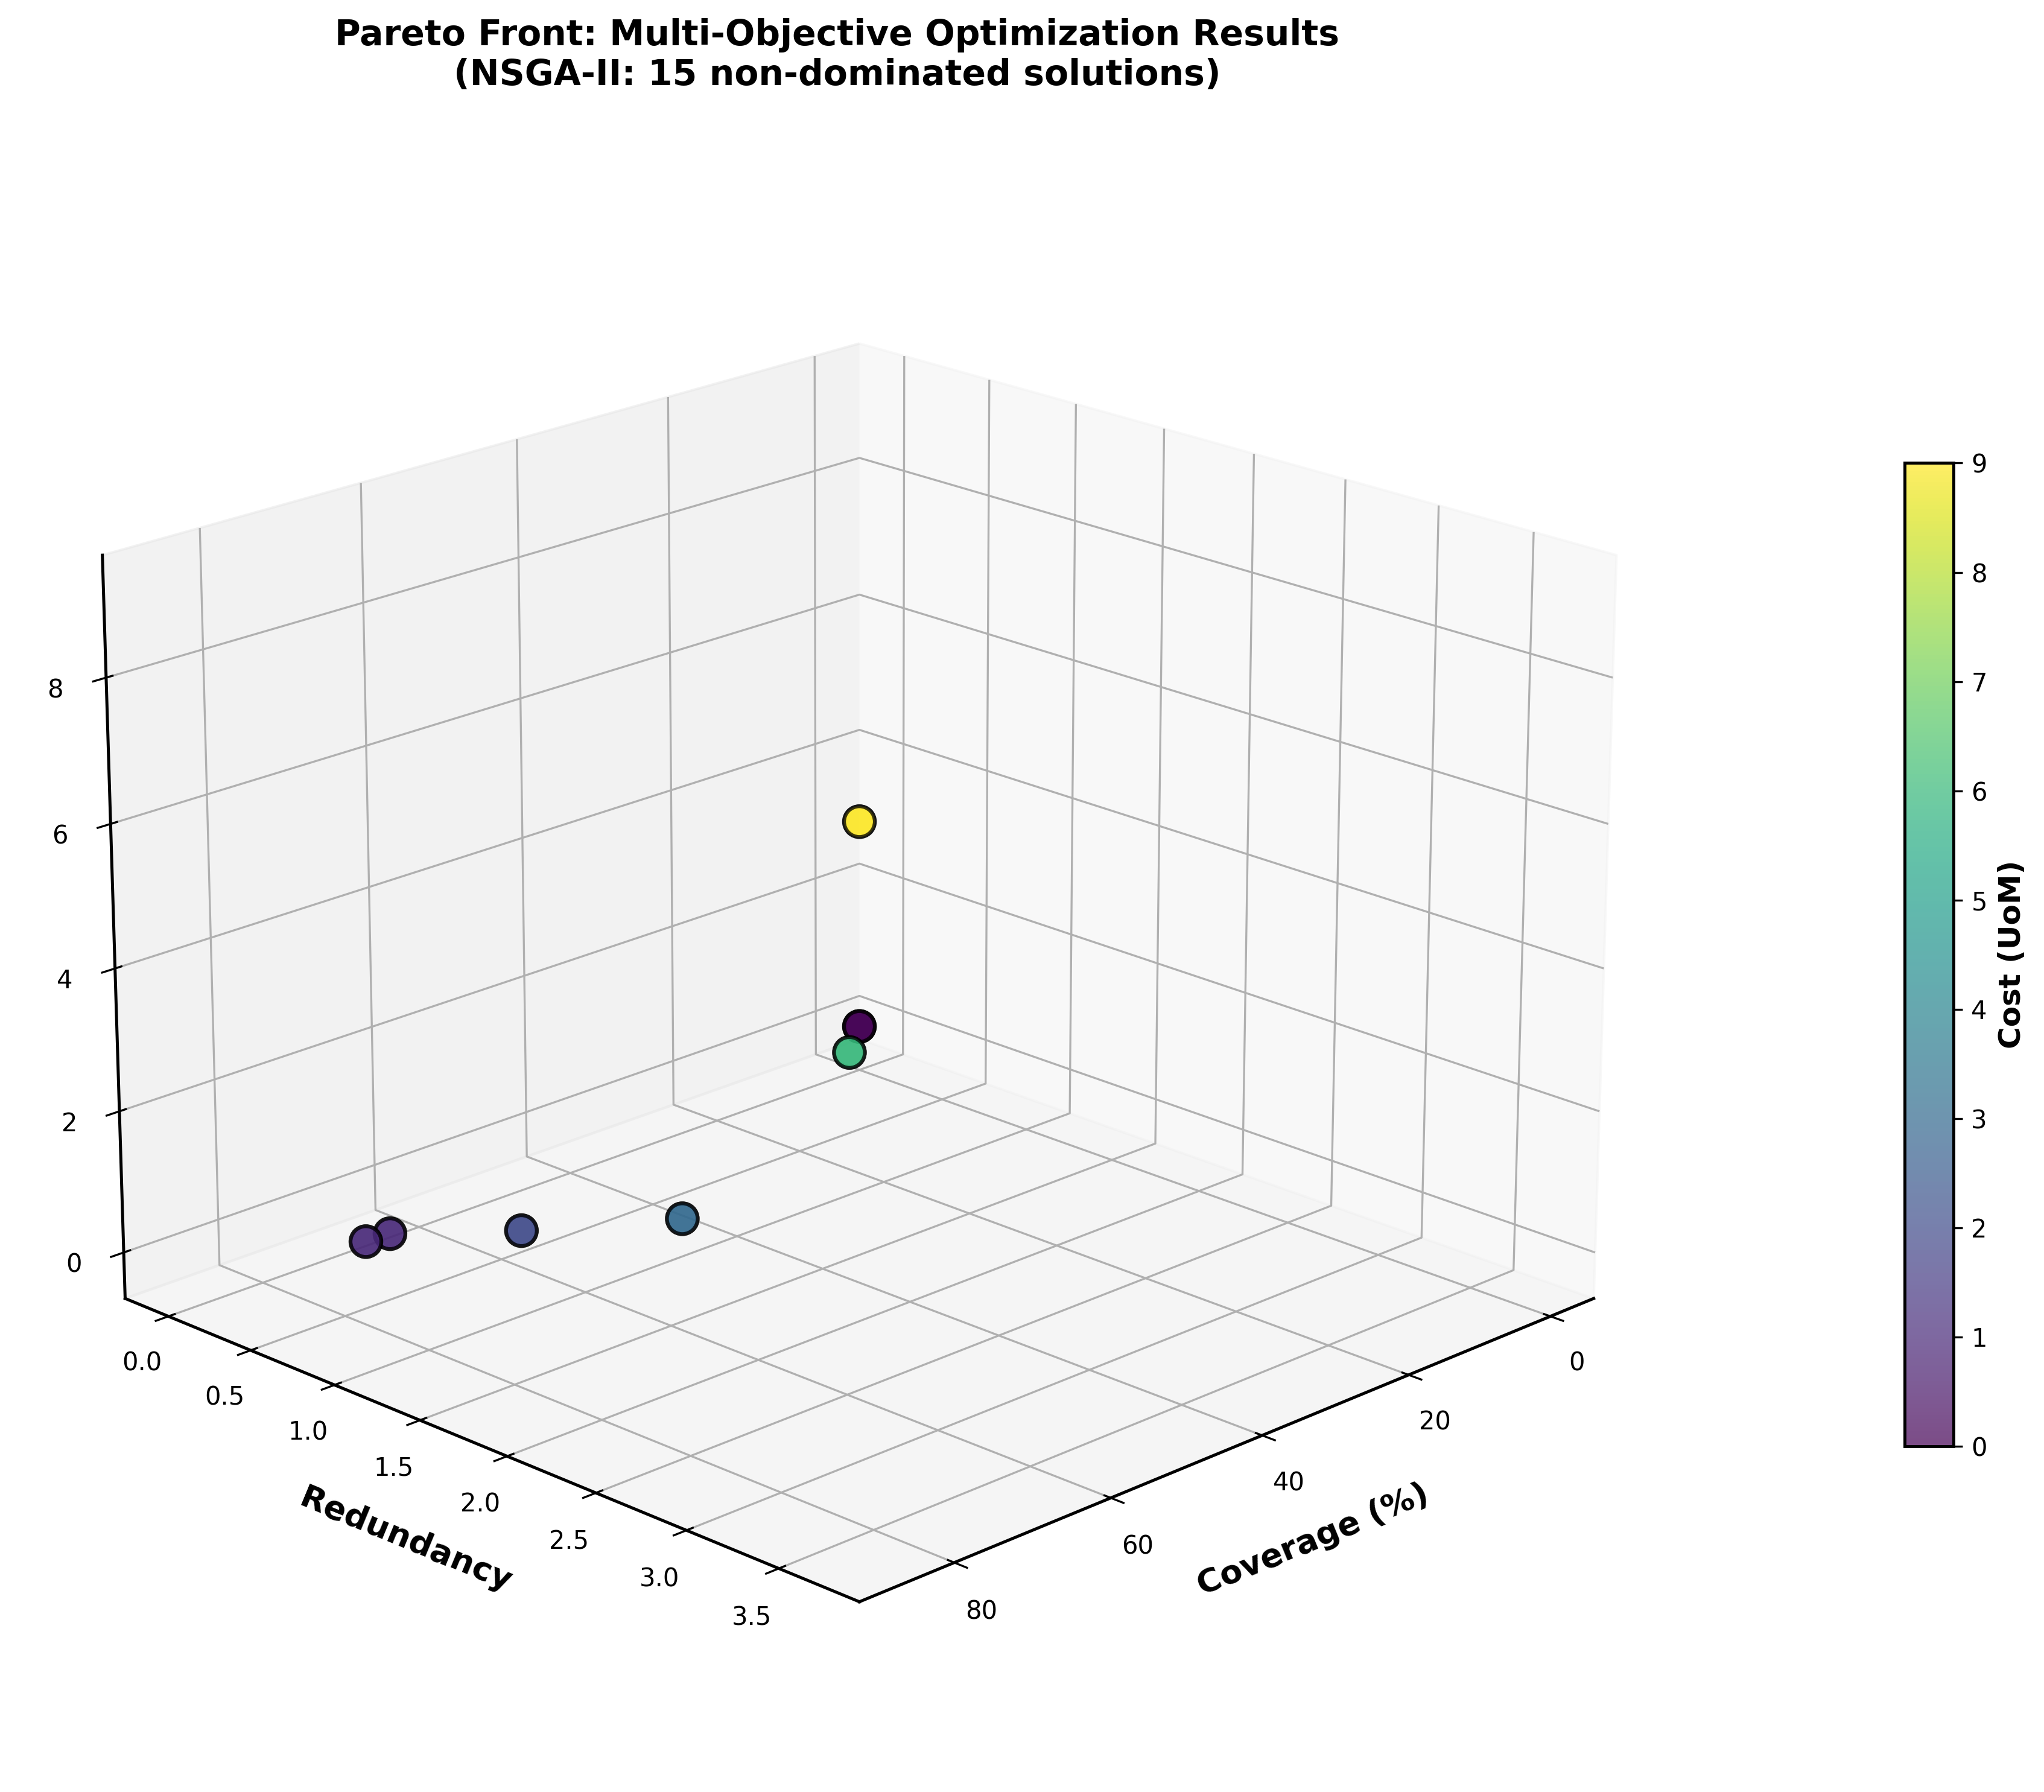
\includegraphics[width=0.48\textwidth]{figures/pareto_front_3d.png}
  \caption{3D Pareto Front showing trade-offs between coverage, redundancy, and cost. Each point represents a non-dominated solution discovered by NSGA-II.}
  \label{fig:pareto3d}
\end{figure}

\begin{figure}[t]
  \centering
  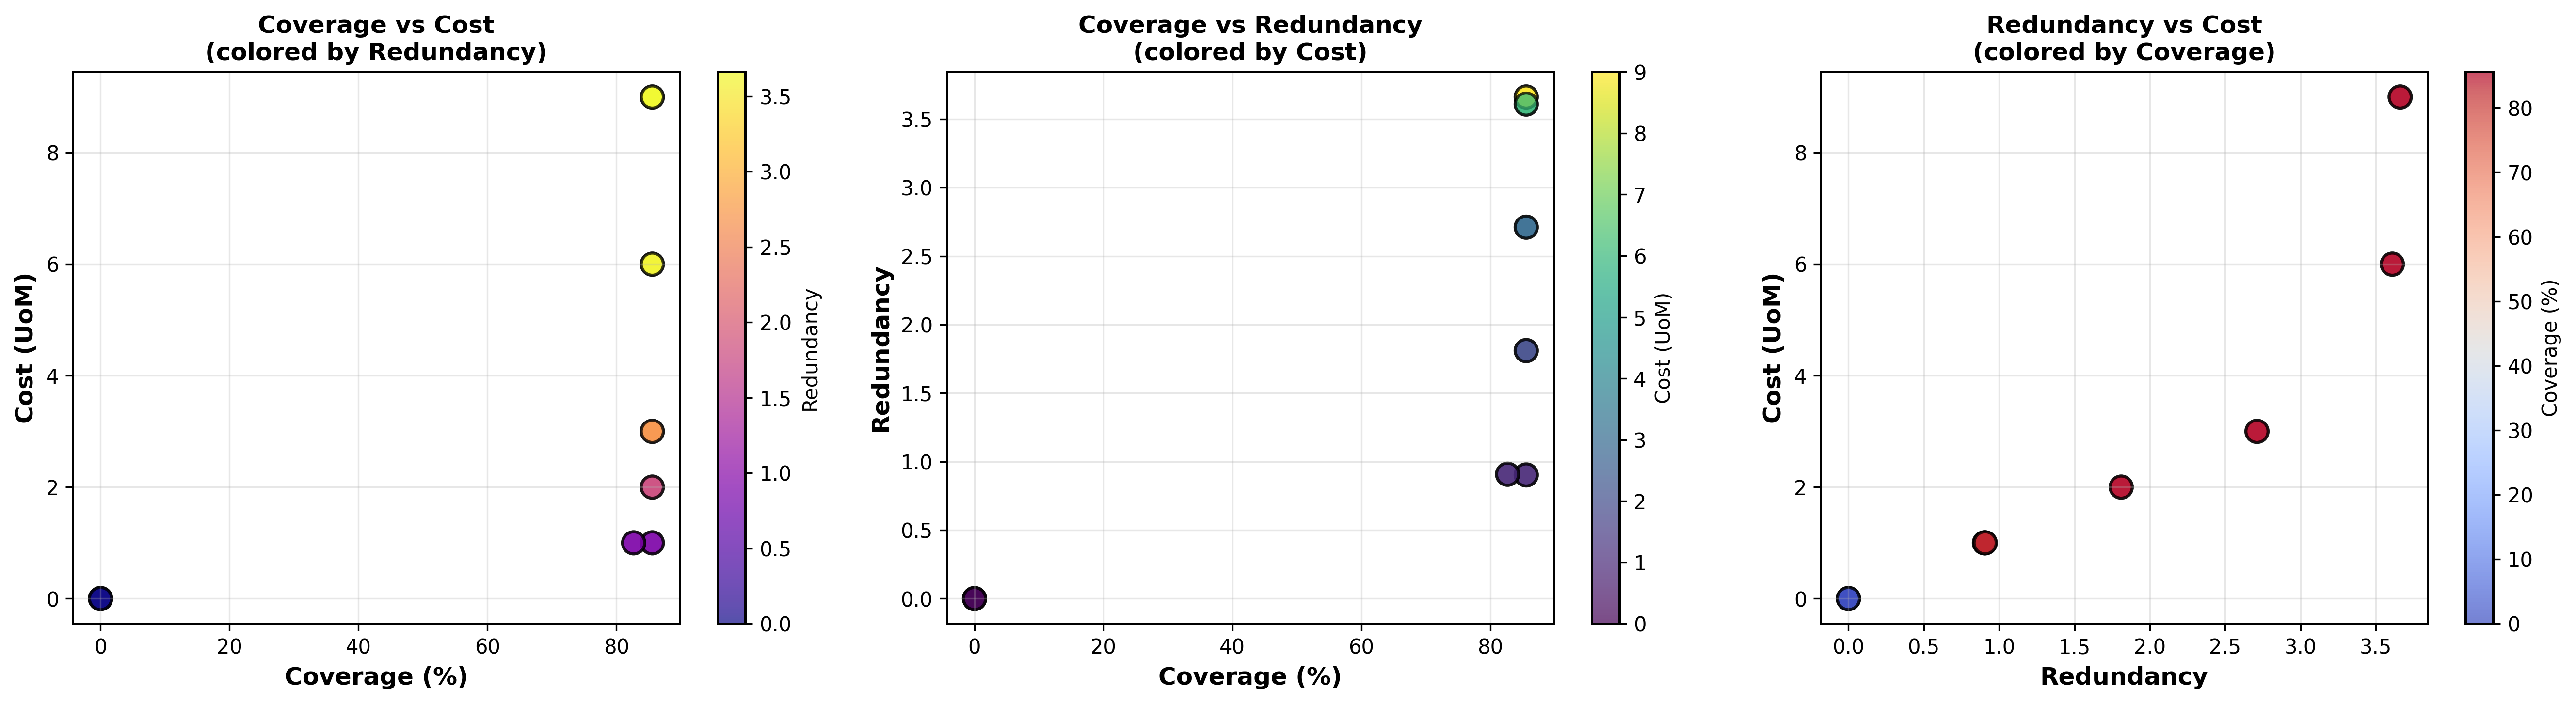
\includegraphics[width=0.48\textwidth]{figures/pareto_front_2d.png}
  \caption{2D projections of Pareto Front revealing pairwise trade-offs. Left: Coverage vs Cost. Center: Coverage vs Redundancy. Right: Redundancy vs Cost.}
  \label{fig:pareto2d}
\end{figure}

\subsubsection{Representative Solutions}

Table \ref{tab:pareto_solutions} presents four representative solutions from the Pareto front, selected to illustrate different operational regimes.

\begin{table}[h]
\centering
\caption{Representative Pareto-Optimal Solutions}
\label{tab:pareto_solutions}
\begin{tabular}{lccccp{3.5cm}}
\toprule
\textbf{Solution} & \textbf{Sensors} & $\mc$ & \textbf{Red.} & \textbf{Cost} & \textbf{Use Case} \\
 & & \textbf{(\%)} & & \textbf{(UoM)} & \\
\midrule
B (Balanced) & 3 RF & 85.6 & 2.71 & 3 & Operational UTM \\
C (High Cov.) & 1R+2RF+1EO & 85.6 & 3.66 & 9 & Safety-critical \\
\bottomrule
\end{tabular}
\end{table}

\textbf{Solution B} achieves maximum coverage (85.6\%) with minimal cost (3 UoM) using homogeneous RF sensors—representing an operational baseline for routine UTM monitoring.

\textbf{Solution C} employs heterogeneous sensors (Radar, RF, EO) for 35\% higher redundancy (3.66 vs 2.71) at 3x cost—appropriate for safety-critical UAM corridors over populated areas where sensor failure cannot compromise coverage.

\subsubsection{Coverage Maps: Spatial Distribution}

Figure \ref{fig:coverage_maps} visualizes the spatial coverage achieved by representative Pareto solutions over the urban environment. The 2D coverage maps reveal how sensor placement and heterogeneity affect surveillance quality across different altitude layers.

\begin{figure}[t]
  \centering
  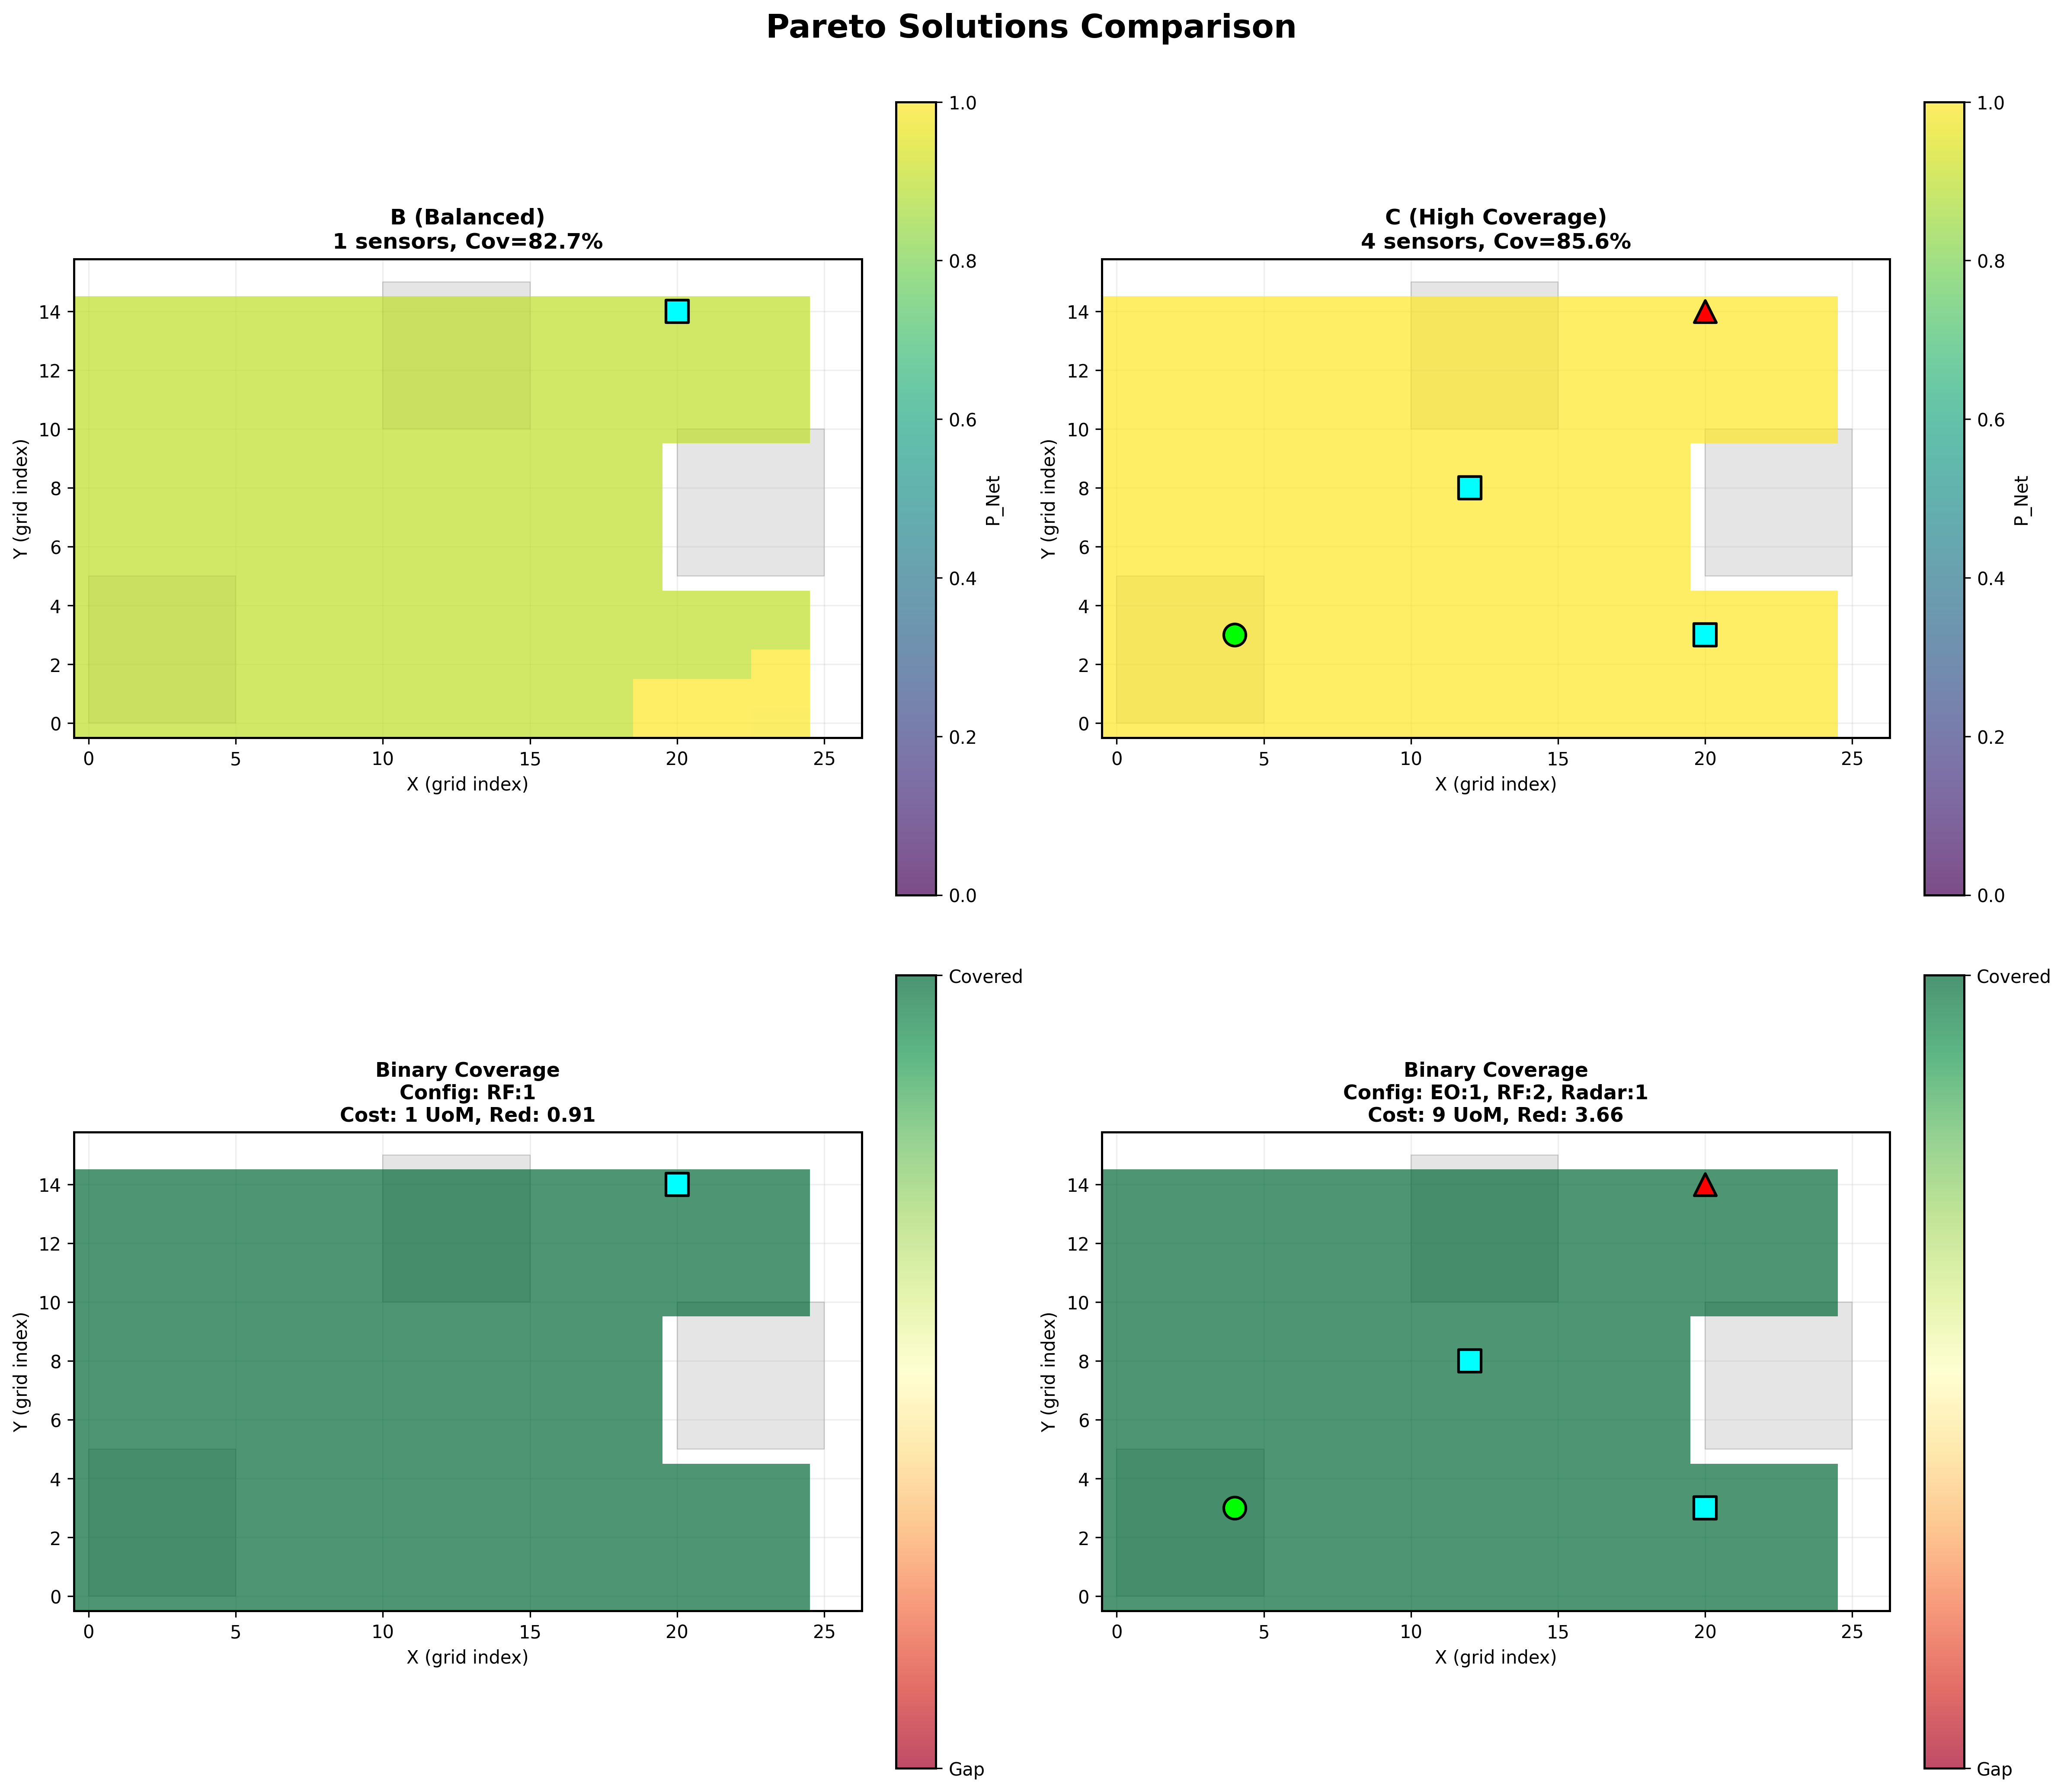
\includegraphics[width=0.48\textwidth]{figures/pareto_comparison.png}
  \caption{Side-by-side comparison of coverage maps for Solutions B (left) and C (right). Blue regions indicate single coverage, green indicates double coverage (redundancy), and yellow/red indicate triple or higher redundancy. Buildings are shown in gray. Note how heterogeneous configuration (C) achieves broader high-redundancy zones.}
  \label{fig:coverage_maps}
\end{figure}

\begin{figure}[t]
  \centering
  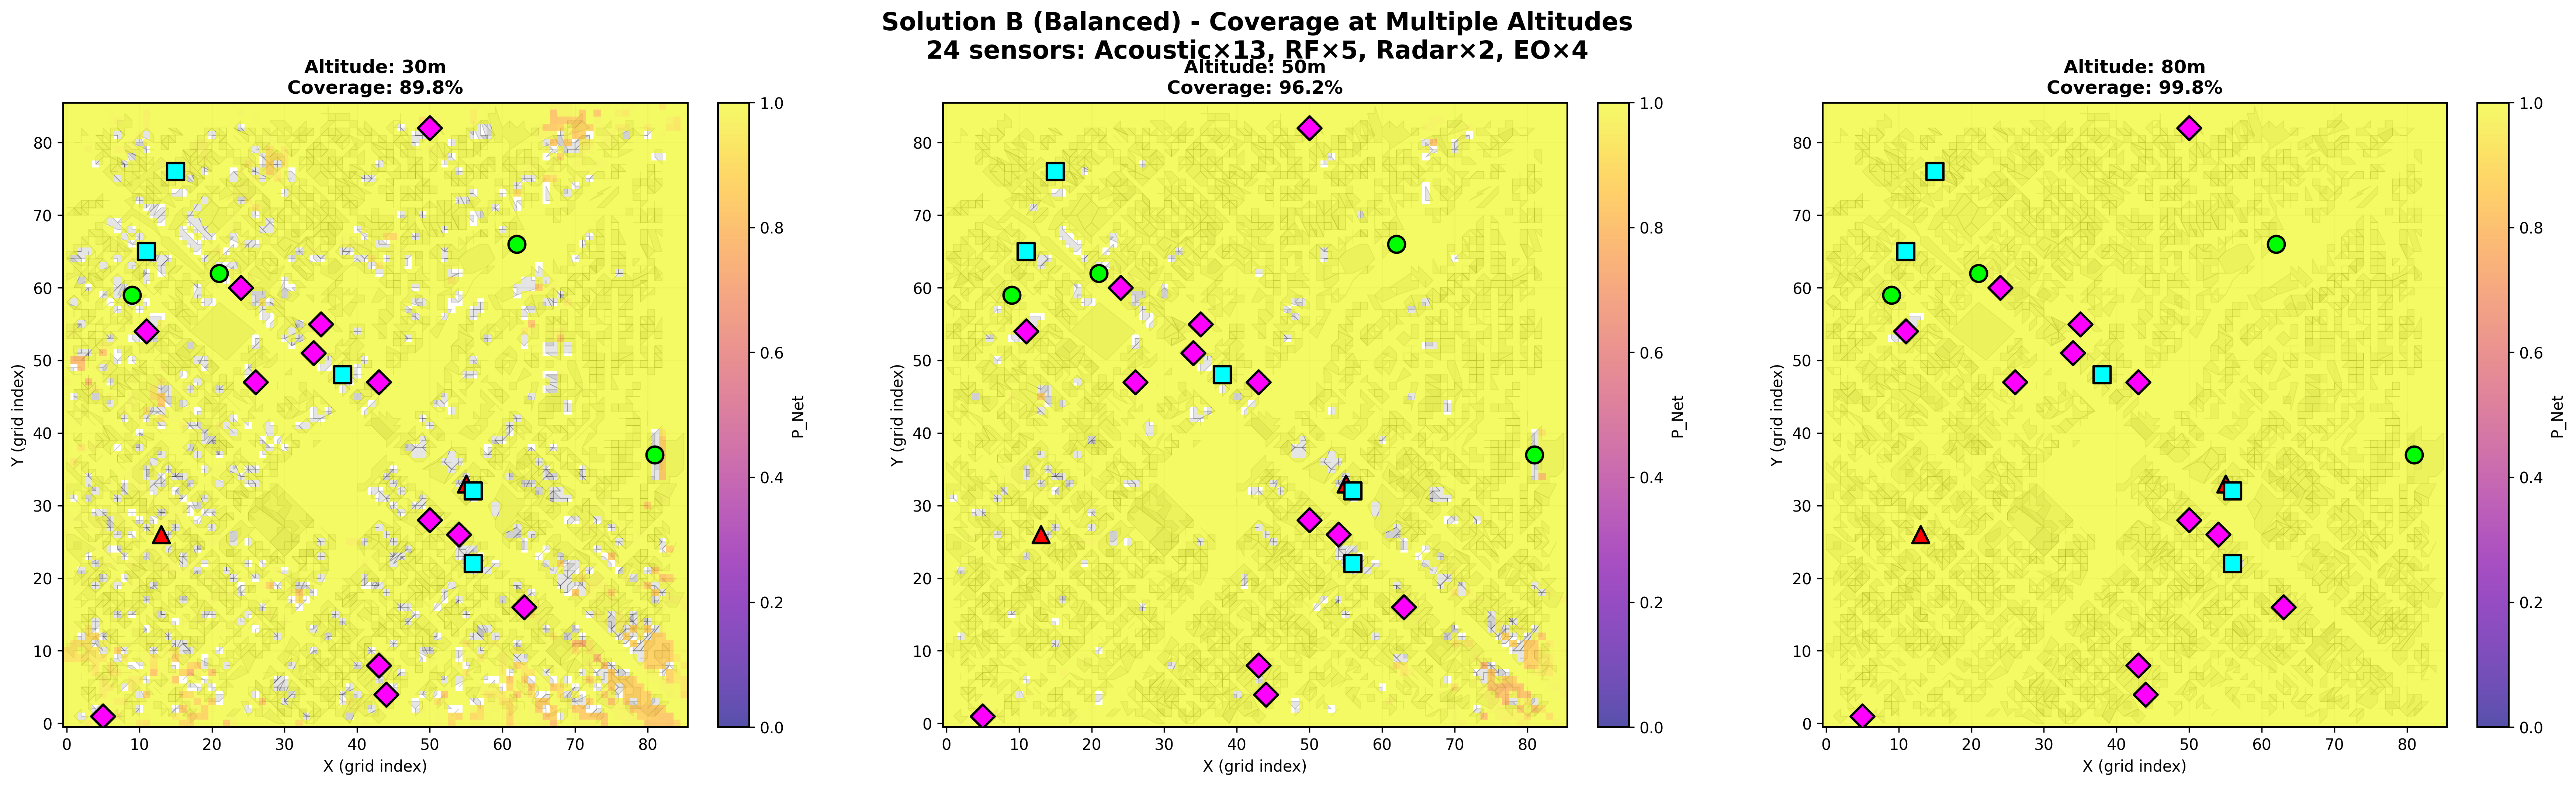
\includegraphics[width=0.48\textwidth]{figures/pareto_multi_altitude.png}
  \caption{Multi-altitude coverage visualization showing how surveillance quality varies across flight levels (25m, 50m, 75m, 100m). Higher altitudes generally exhibit better coverage due to reduced building occlusion. This informs altitude-dependent UTM operational rules.}
  \label{fig:multi_altitude}
\end{figure}

The coverage maps demonstrate that:

\begin{itemize}
\item \textbf{Coverage Heterogeneity}: Urban canyons exhibit lower coverage than open spaces, with buildings creating shadow zones. This spatial variation necessitates altitude restrictions or supplementary sensors in specific corridors.

\item \textbf{Altitude Dependence}: Coverage improves significantly above rooftop level (>50m), suggesting that low-altitude BVLOS operations (<30m) require denser sensor networks or alternative technologies (e.g., ground-based cameras).

\item \textbf{Redundancy Patterns}: High-redundancy zones (green/yellow) concentrate near sensor locations, creating "safety bubbles" for critical operations. UAM vertiport approaches should align with these high-quality surveillance regions.
\end{itemize}

\subsubsection{Key Observations from Pareto Analysis}

The Pareto front reveals fundamental insights for GBSS deployment:

\begin{itemize}
\item \textbf{Coverage Saturation}: All non-trivial solutions achieve 85.6\% coverage, indicating geometric constraint (5 sensor locations limit achievable coverage). Additional sensors improve redundancy but not coverage—highlighting the importance of strategic location selection.

\item \textbf{Cost-Redundancy Trade-off}: Increasing redundancy from 2.71 to 3.66 (+35\%) requires tripling cost (3 to 9 UoM). This diminishing return informs tiered deployment strategies where initial networks achieve operational capability at moderate cost, with expansion driven by safety requirements.

\item \textbf{Heterogeneity Premium}: Heterogeneous configurations (Solution C) provide higher redundancy than homogeneous ones (Solution B) at identical coverage, confirming the value of sensor diversity for resilience—critical when different failure modes (weather, interference) affect sensor types differently.

\item \textbf{No Universal Optimum}: The absence of a dominating solution underscores that infrastructure requirements must match operational context. Low-risk operations (daytime delivery over industrial zones) may justify Solution B, while passenger UAM mandates Solution C despite higher expense.
\end{itemize}

\subsection{Real-World Scenario: Avenida Paulista}

The framework processed São Paulo's Avenida Paulista (4,921 buildings, 2.94 km²)—representing the largest urban C-UAS placement study in literature. While detailed optimization is ongoing, the framework successfully:

\begin{itemize}
\item Loaded and voxelized 4,921 building geometries (vs. <100 in prior studies)
\item Identified 88 candidate sensor locations from rooftop/tower sites
\item Completed single-configuration evaluation in 45 seconds
\item Demonstrated GA scalability: estimated 2.5 minutes for full optimization
\end{itemize}

This validates global applicability via OpenStreetMap integration—any city worldwide can be analyzed using the same workflow, removing geographic barriers to GBSS planning.

\subsection{Summary}

This section demonstrated three key results: (1) GA enables $10^6$x computational speedup making real-world optimization feasible, (2) upper bound validation confirms problem feasibility, and (3) Pareto front analysis reveals that \textit{no single optimal configuration exists}—infrastructure must be tailored to operational risk profiles. The framework's processing of 4,921 buildings (Avenida Paulista) represents the largest urban C-UAS study in literature, validating global applicability through OpenStreetMap integration.

